

\subsection{Пример использования}


Для демонстрации работы приложения был создан небольшой бот, который
просит ввести пользователя код HTTP статуса ответа и после выводит соответствующую картинку
с котом. Для получения картинок использовался сервис https://http.cat/.
Экранные формы примера работы приложения представлены на рисунках~
\ref{f:example:bot-struct}-\ref{f:example:telegram-2}.

\begin{figure}[H]
	\centering
	\vspace{\toppaddingoffigure}
	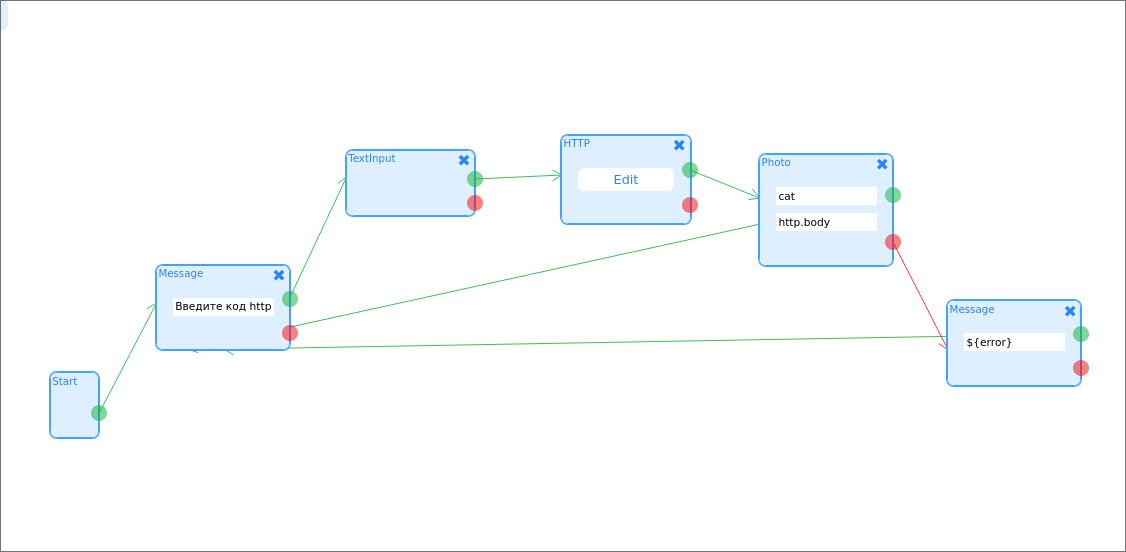
\includegraphics[width=\textwidth]{/example/bot-struct}
	\caption{Построение структуры бота}
	\label{f:example:bot-struct}
\end{figure}


\begin{figure}[H]
	\centering
	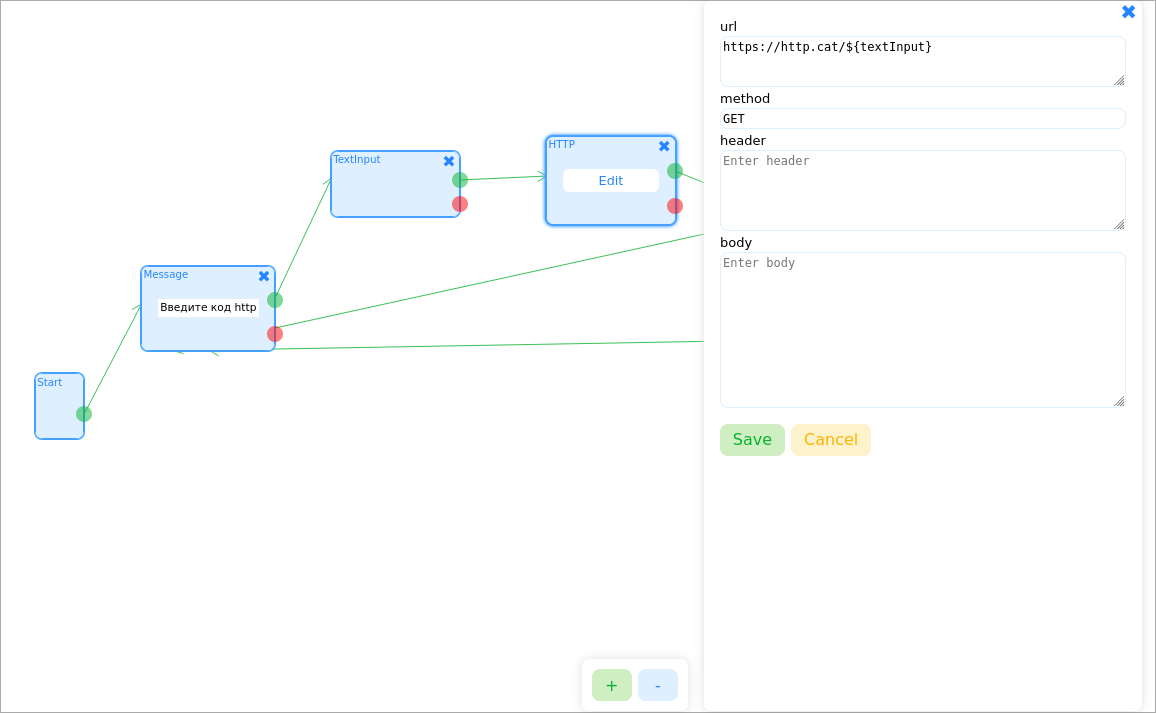
\includegraphics[width=\textwidth]{/example/http-setup}
	\caption{Настройка HTTP компонента}
	\label{f:example:http-setup}
\end{figure}

\begin{figure}[H]
	\centering
	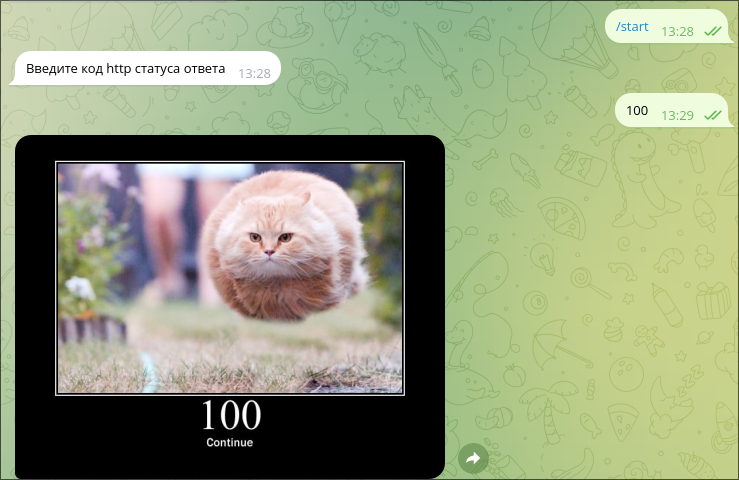
\includegraphics[width=0.9\textwidth]{/example/telegram-1}
	\caption{Использование созданного бота}
	\label{f:example:telegram-1}
\end{figure}


\begin{figure}[H]
	\centering
	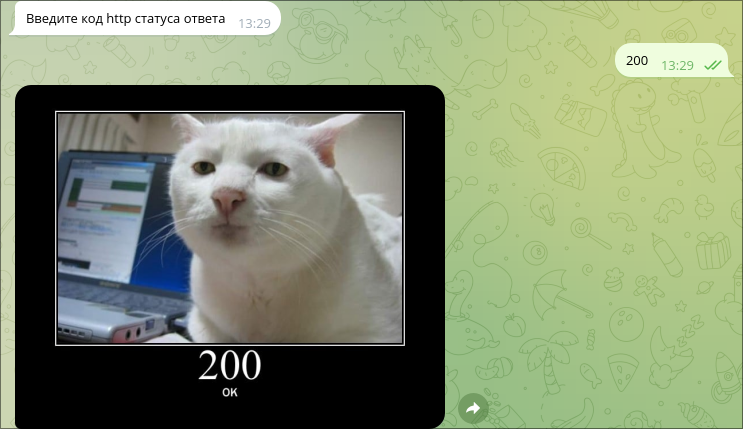
\includegraphics[width=0.9\textwidth]{/example/telegram-2}
	\caption{Использование созданного бота}
	\label{f:example:telegram-2}
\end{figure}
